\usepackage{listingsutf8}
\usepackage[utf8]{inputenc}
\usepackage[T1]{fontenc}
\usepackage{xcolor}
\usepackage{hyperref}

\usetheme{CambridgeUS}
\title{Git a look under the hood}
\subtitle{Build a deeper understanding of gits internals}
\author{Vincent Scherb}
\institute{IPI GmbH}
\date{\today}
\logo{
\includegraphics[height=1cm]{images/ipi-logo.png}}

% source: https://tex.stackexchange.com/questions/46953/unix-command-highlighting-latex/46994#46994
\lstdefinestyle{BashInputStyle}{
    language=bash,
    basicstyle=\small\ttfamily,
    numbers=left,
    numberstyle=\tiny,
    numbersep=3pt,
    frame=tb,
    columns=fullflexible,
    backgroundcolor=\color{yellow!20},
    linewidth=0.9\linewidth,
    xleftmargin=0.1\linewidth
}

\begin{document}
    \frame{\titlepage}

    \section*{Table of Contents}
    \begin{frame}
        \frametitle{Table of Contents}
        \tableofcontents
    \end{frame}

    \section{Contents of .git directory}
\begin{frame}[fragile]
    \frametitle{Exploring the .git directory}
    \begin{figure}
        \begin{center}
            \ifnumequal{\aspectratio}{43}
            {
                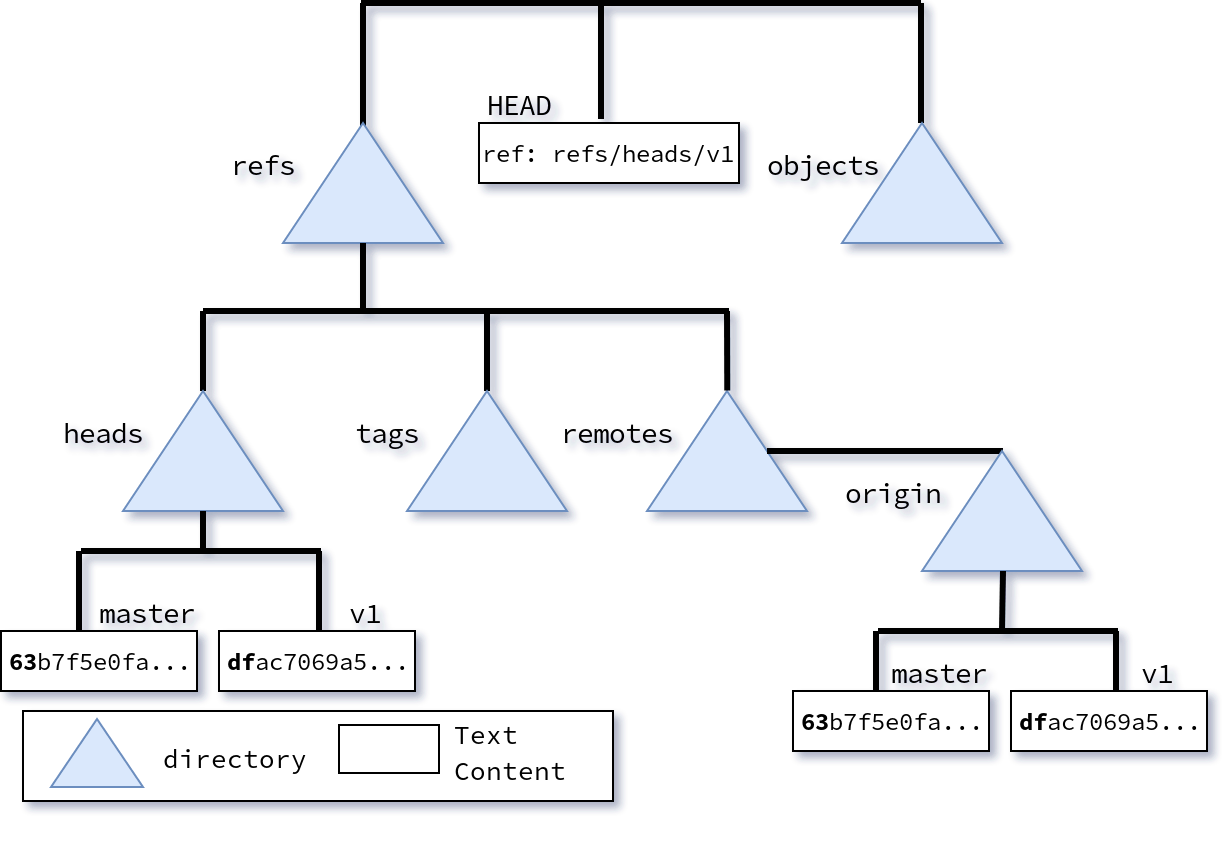
\includegraphics[height=0.75\textheight,keepaspectratio]{./images/gitDirectory.png}
            }
            {
                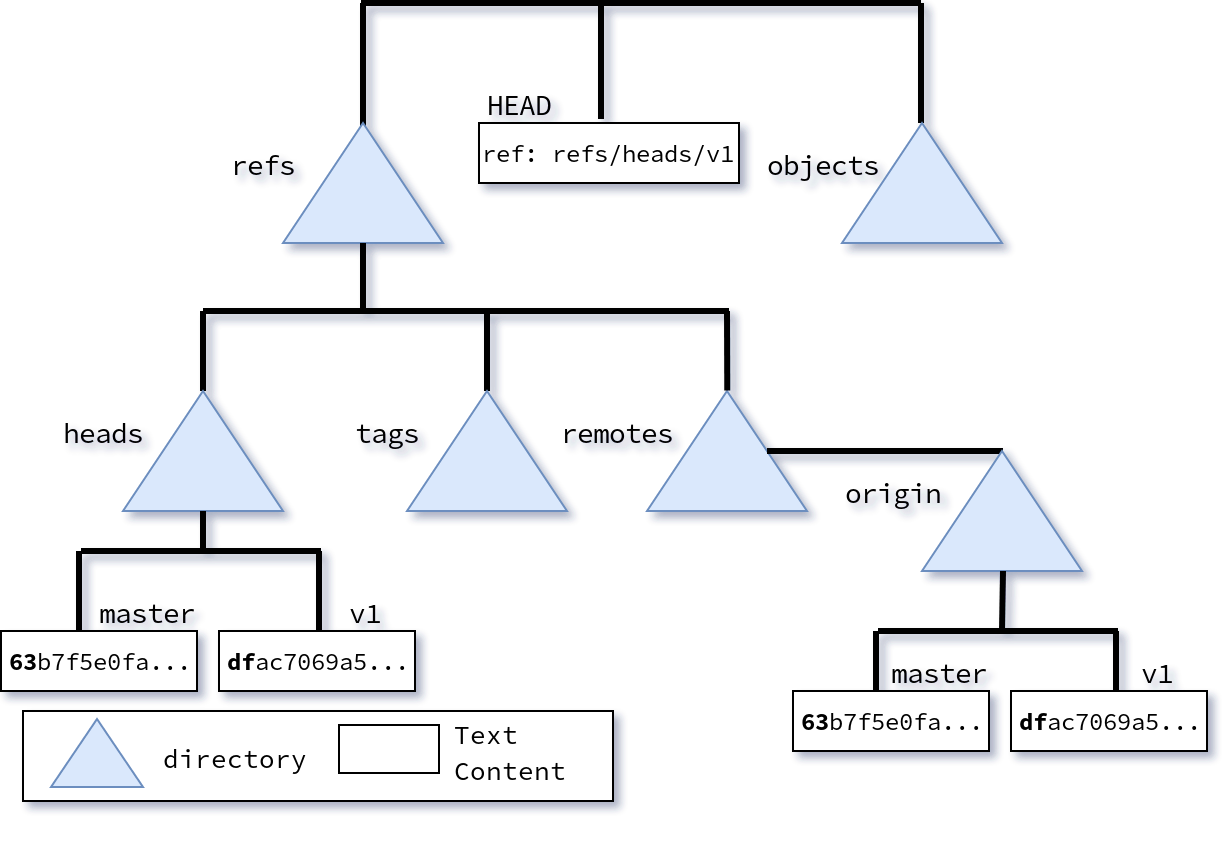
\includegraphics[height=0.75\textheight,width=0.8\textwidth]{./images/gitDirectory.png}
            }
            \caption{.git directory}
        \end{center}
    \end{figure}
\end{frame}



\end{document}

